\section{Algoritmo exacto para cografo y grafo completo}

% El nuevo problema que tienen Marty y el Doc es que ahora no se ponen de
% acuerdo en qué estructura quı́mica deben utilizar para armar el condensador
% de flujos. Marty, a partir de las propiedades atómicas, ha obtenido una
% constante n y está seguro de que la solución que están buscando debe ser un
% grafo de a lo sumo n vértices (o como él lo dice, un subgrafo de algún Kn),
% mientras que el Doc ha estudiado las caracterı́sticas moleculares e insiste
% con que debe ser un subgrafo de un cografo dado. Por las dudas, y para
% evitar más conflictos entre ellos, quieren cumplir con ambas
% especificaciones, siempre maximizando la cantidad de aristas, dado que éste
% es el punto clave para su funcionamiento dentro del condensador. Por eso les
% pedimos que los ayuden diseñando e implementando un algoritmo exacto para
% MCS que tenga complejidad temporal polinomial para el caso en el que G1 es
% un cografo y G2 es un grafo completo y desarrollen los siguientes puntos que
% avalen la solución encontrada (si estamos hablando de viajar en el tiempo,
% no hay margen de error posible):
% a) Explicar detalladamente el algoritmo implementado.
% b) Calcular el orden de complejidad temporal de peor caso del algoritmo.
% c) Realizar una experimentación que permita observar los tiempos de
%    ejecución del algoritmo en función del tamaño de entrada.

\subsection{Introducción}
En este ejercicio, se busca encontrar un algoritmo exacto para resolver, en
tiempo polinomial, el problema del \acr{MCS} entre dos grafos cuando uno de
ellos es un grafo completo y el otro es un \emph{cografo}. La clase de los
cografos, o grafos reducibles por complemento, se define recursivamente y
consiste exactamente en los grafos que pueden construirse según alguna de las
siguientes reglas:
\begin{enumerate}
    \item Un nodo aislado ($K_1$) es un cografo.
    \item La unión de dos o más cografos es un cografo.
    \item El complemento de un cografo es un cografo.
\end{enumerate}

Es posible demostrar (\cite{corneil}, Corneil et al.) que todo cografo
admite una representación mediante un árbol enraizado, que se conoce como
coárbol (o \emph{cotree}) del mismo. Existen diferentes variantes de esta
representación, pero en todas ellas las hojas del árbol corresponden a los
nodos del grafo, mientras que los nodos internos representan el cografo que se
obtiene aplicando una determinada operación a los cografos relativos a sus
nodos hijos. Así, la raíz del coárbol se corresponde con el cografo completo
que se busca representar.

% Para obtener esta representación se parte de que todo cografo, o bien es una
% unión disjunta de cografos, o su complemento lo es. De esto se sigue que
% todo cografo puede reducirse a un conjunto de nodos aislados complementando
% de forma sucesiva sus componentes conexas (de allí que a estos grafos se los
% conozca como \emph{reducibles por complemento}). Esto equivale a decir que
% puede darse una forma iterativa para construir cualquier cografo a partir de
% sus nodos; se comienza considerando todos ellos como grafos disjuntos, y
% luego se conectan estos grafos iterativamente computando en cada paso el
% complemento de la unión de algunos de ellos. Dado un cografo cualquiera, su
% coárbol no es más que la representación de este proceso mediante un árbol:
% las hojas del mismo corresponden a los nodos del cografo, y cada nodo
% interno representa el complemento de la unión de los cografos
% correspondientes a sus hijos. El cografo en sí mismo es representado la raíz
% del árbol.

En este trabajo, las dos operaciones que se utilizarán para etiquetar los
nodos internos de un coárbol provienen de una definición alternativa y
equivalente de cografo: un grafo es un cografo si y solo si puede obtenerse a
partir de nodos aislados mediante la aplicación sucesiva de la unión disjunta
($\cup$) y el \emph{join} ($\times$). Esta última operación se define de la
siguiente forma: dados $G_1, \dots, G_k$ grafos, el \emph{join} entre ellos es
el grafo $G_1 \times \dots \times G_k = \left((G_1)\comp \cup
\dots \cup (G_k)\comp\right)\comp$. Una forma más intuitiva de pensar el
\emph{join} entre grafos es partir de la unión disjunta entre ellos, y agregar
todas las aristas cuyos extremos se encontraban en grafos distintos.

Otra consideración a tener en cuenta es que, para simplificar la
implementación, se utilizarán coárboles estrictamente binarios; es decir,
cada nodo interno representará una operación entre exactamente dos cografos.
Esto no resulta problemático, ya que tanto la unión como el \emph{join} entre
grafos son operaciones asociativas.

\begin{figure}[htbp]
    \centering
    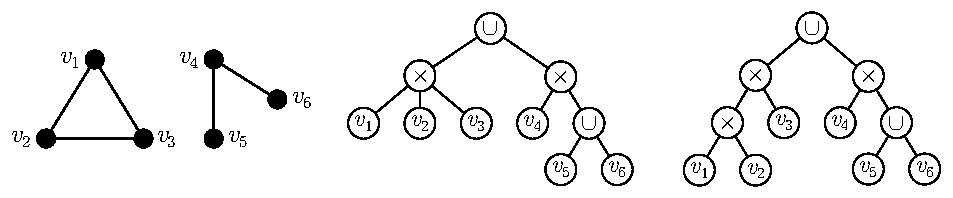
\includegraphics{imagenes/ex3_ejemplo-coarbol.pdf}
    \caption{Ejemplo de un cografo, su coárbol correspondiente, y la
    representación estrictamente binaria del mismo.}
    \label{fig:cografos:ejemplo-coarbol}
\end{figure}

\subsection{Resolución algorítmica}
Sean $G_1$ un cografo con $N_1$ nodos y $M_1$ aristas, y $G_2 = K_{N_2}$ un
grafo completo de $N_2$ nodos (que tendrá por lo tanto $M_2 = \frac{N_2 \times
(N_2 - 1)}{2}$ aristas). A la hora de resolver el problema de encontrar el
\acr {MCS} entre $G_1$ y $G_2$, pueden distinguirse estos dos casos:
\begin{enumerate}
    \item $N_1 \leq N_2$. Dado que $G_2$ es un grafo completo, todo
    subgrafo que tenga $N_2$ o menos nodos, y en particular $G_1$,
    es isomorfo a algún subgrafo de $G_2$. Como, trivialmente, $G_1$ es
    isomorfo a sí mismo, basta tomar $G_1$ como solución del problema.
    \item $N_1 > N_2$. Para resolver este caso del problema, basta con
    tomar un subgrafo inducido de $G_1$ que tenga exactamente $N_2$ nodos y
    maximice la cantidad de aristas.

    En efecto, sea $H$ un grafo isomorfo a algún subgrafo de $G_1$. Para ser
    solución de \acr{MCS}, $H$ debe resultar isomorfo a algún subgrafo de
    $G_2$, lo cual sucede si y solo si su cantidad de nodos es menor o igual
    que $N_2$. Si $H$ tiene menos de $N_2$ nodos, puede extenderse a algún
    grafo $\tilde{H} \supseteq H$ que tenga exactamente $N_2$ nodos y también
    sea isomorfo a un subgrafo de $G_1$. Es directo que $\tilde{H}$ resulta
    isomorfo a algún subgrafo de $G_2$ y que su cantidad de aristas es mayor o
    igual que la de $H$. Entonces, si $H$ era solución óptima de
    \acr{MCS}, claramente $\tilde{H}$ también lo es.

    Por otra parte, todo subgrafo de $H \subseteq G_1$ que sea solución de
    \acr{MCS} es necesariamente un subgrafo inducido; en caso contrario,
    pueden agregarse las aristas faltantes para convertirlo en un subgrafo
    inducido $\tilde{H}$, que también será isomorfo a subgrafos de $G_1$ y
    $G_2$ pero tendrá más aristas que $H$, contradiciendo la hipótesis de que
    este último tenía una cantidad de aristas máxima.
\end{enumerate}

Dado que la resolución del primer caso es trivial, durante el resto de esta
sección se asumirá que $N_1 > N_2$. Se llamará $G = G_1$, $N = N_1$, $M = M_1$
y $K = N_2$, y se explicará la solución planteada al problema de encontrar un
subgrafo inducido de un cografo $G$ que tenga exactamente $K$ vértices y
cantidad de aristas máxima. Aprovechando la hipótesis de que $G$ es un
cografo, es posible solucionar el problema en tiempo polinomial.

La solución propuesta tiene dos etapas. En primer lugar, se crea el coárbol
binario de $G$, y luego, utilizando la técnica de programación dinámica, se
aprovecha esta representación para obtener el subgrafo buscado.

% \begin{lema} Sea $G$ un cografo. Si $H \subseteq G$ es un subgrafo inducido
% no vacío de $G$, entonces $H$ es un cografo. Además:
% \begin{enumerate}
%     \item Si $G = K_1$, entonces $H = K_1$.
%     \item Si $G = G_1 \cup G_2$, entonces $H = H_1$, $H = H_2$ o $H = H_1
%     \cup H_2$, siendo $H_1$ y $H_2$ subgrafos inducidos de $G_1$ y $G_2$,
%     respectivamente.
%     \item Si $G = G_1 \times G_2$, entonces $H = H_1$, $H = H_2$ o $H = H_1
%     \times H_2$, siendo $H_1$ y $H_2$ subgrafos inducidos de $G_1$ y $G_2$,
%     respectivamente.
% \end{enumerate}
% \end{lema}
% \begin{proof}
% Por inducción estructural, utilizando la definición recursiva de cografo.
% \begin{enumerate}
%     \item Caso base: $G = K_1$. En este caso, necesariamente, $H = K_1$, que
%     es un cografo.
%     \item Caso recursivo: $G = G_1 \cup G_2$ con $G_1$ y $G_2$ cografos. Se
%     supone, por hipótesis inductiva, que todo subgrafo inducido de los mismos
%     es, a su vez, un cografo. Existen dos posibilidades:
%     \begin{enumerate}
%         \item $H$ es subgrafo inducido de $G_1$ o de $G_2$, en cuyo caso la
%         hipótesis inductiva asegura que $H$ es un cografo.
%         \item Hay nodos de $H$ tanto en $G_1$ como en $G_2$. En tal caso, sean
%     $H_1$ y $H_2$ los subgrafos inducidos en $G_1$ y $G_2$, respectivamente,
%     por los nodos correspondientes de $H$. Por hipótesis inductiva, $H_1$ y
%     $H_2$ son cografos. Se demostrará que $H = H_1 \cup H_2$. Claramente los
%     conjuntos de vértices coinciden. En cuanto a los conjuntos de aristas, se
%     probará que dados $v_1, v_2 \in V(H) = V(H_1, H_2)$, $(v_1, v_2) \in E(H)
%     \Leftrightarrow (v_1, v_2) \in E(H_1 \cup H_2)$.
%         \begin{itemize}
%             \item[($\Rightarrow$)] $(v_1, v_2) \in E(H)$.
%         \end{itemize}
%     \end{enumerate}
%     \item Caso recursivo: $G = G_1 \times G_2$ con $G_1$ y $G_2$ cografos. Es
%     análogo al caso anterior.
% \end{enumerate}
% \end{proof}

\subsubsection{Construcción del coárbol}
Para construir el coárbol correspondiente a un cografo dado, se descompone el
mismo en cografos de menor tamaño hasta obtener un conjunto de vértices
aislados. El algoritmo admite una sencilla formulación recursiva: si el
cografo consiste en un vértice aislado, el coárbol tendrá un único nodo
representando este vértice. En caso contrario, el cografo será la unión o el
\emph{join} de dos cografos; el coárbol que lo represente tendrá como raíz un
nodo etiquetado con esa operación, del cual colgarán los coárboles
correspondientes a los dos cografos sobre los cuales esta se aplica.

La implementación propuesta adapta esta formulación para que resulte
iterativa. El proceso que se lleva a cabo se puede interpretar de la siguiente
forma: se parte de un árbol con un único nodo, que representa al cografo
completo. En cada paso, se toma una hoja de este árbol y, si el cografo que
representa es la unión o el \emph{join} de dos cografos, se la reemplaza por
un nodo indicando dicha operación, con dos hijos representando a estos dos
cografos. A continuación, estas dos nuevas hojas se encolan para ser
procesadas más adelante. El proceso se repite hasta que todas las hojas del
árbol hayan sido reducidas a un grafo trivial.

El pseudocódigo del algoritmo planteado se presenta como Algoritmo
\ref{alg:ex3:coarbol}.

\bigskip
\begin{algorithm}[H]
    \SetAlgoVlined
    \caption{Construcción del coárbol correspondiente a un cografo}
    \label{alg:ex3:coarbol}
    \Input{Un cografo $G = (V, E)$ con $N$ nodos y $M$ aristas, representado
    como listas de adyacencia.}
    \Output{El coárbol binario correspondiente a $G$.}

    $G\comp$ $\gets$ complemento de $G$ \;
    \textit{nodo\_inicial} $\gets$
    $\langle$subgrafo: $G$, padre: \textsf{ninguno}, lado: \textsf{ninguno}$\rangle$ \;
    \textit{a\_expandir} $\gets$ cola de nodos vacía \;
    \textit{a\_expandir}.encolar(\textit{nodo\_inicial}) \;

    \While{\textit{a\_expandir} no esté vacía} {
        \textit{subgrafo\_actual} $\gets$ \textit{a\_expandir}.desencolar().subgrafo \;
        \textit{padre\_actual} $\gets$ \textit{a\_expandir}.desencolar().padre \;
        \textit{lado\_actual} $\gets$ \textit{a\_expandir}.desencolar().lado \;
        $cc_1$ $\gets$ componente conexa de ($G$ restringido a) \textit{subgrafo\_actual} \;
        \eIf{$cc_1$ tiene la misma cantidad de nodos que \textit{subgrafo\_actual}} {
            $cc_1$ $\gets$ componente conexa de ($G\comp$ restringido a) el complemento de \textit{subgrafo\_actual} \;
            \textit{operación} $\gets$ $\times$ \;
        } {
            \textit{operación} $\gets$ $\cup$ \;
        }
        $cc_2$ $\gets$ \textit{subgrafo\_actual} $-$ $cc_1$ \;
        \textit{nuevo\_nodo} $\gets$ nodo representando a \textit{operación} \;
        \eIf{\textit{padre\_actual} $=$ \textsf{ninguno}} {
            \textit{raíz\_cotree} $\gets$ \textit{nuevo\_nodo} \;
        } {
            \eIf{\textit{lado\_actual} $=$ \textit{izquierda}} {
                definir \textit{nuevo\_nodo} como hijo izquierdo de \textit{padre\_actual} \;
            } {
                definir \textit{nuevo\_nodo} como hijo derecho de \textit{padre\_actual} \;
            }
        }
        \eIf{$cc_1$ tiene exactamente 1 nodo} {
            definir $cc_1$.obtener\_nodo() como hijo izquierdo de \textit{nuevo\_nodo} \;
        } {
            \textit{a\_expandir}.encolar($\langle cc_1$, \textit{nuevo\_nodo}, \textit{izquierda}$\rangle$) \;
        }
        \eIf{$cc_2$ tiene exactamente 1 nodo} {
            definir $cc_2$.obtener\_nodo() como hijo derecho de \textit{nuevo\_nodo} \;
        } {
            \textit{a\_expandir}.encolar($\langle cc_2$, \textit{nuevo\_nodo}, \textit{derecha}$\rangle$) \;
        }
    }
    \Return{\textit{raíz\_cotree}}
\end{algorithm}
\bigskip

\subsubsection{Búsqueda del subgrafo máximo}
Se llamará $\operatorname{MIS}(G, K)$ al subgrafo de $G$ con $K < N$ nodos que
maximice la cantidad de aristas. Para resolver el problema de encontrar este
subgrafo, se diseñó un algoritmo utilizando la técnica de programación
dinámica. El esquema detrás de la formulación recursiva de este algoritmo es
el siguiente:

\begin{enumerate}
    \item Si $K = 0$, la solución del algoritmo es un grafo sin nodos ni
    aristas.
    \item Si $K > 0$ y $G = K_1$, es decir, un nodo aislado, la solución es
    $K_1$.
    \item Si $G \neq K_1$, entonces existen dos cografos $G_1$ y $G_2$ tales
    que $G = G_1 \cup G_2$ o $G = G_1 \times G_2$. Se busca encontrar un
    subgrafo inducido $H \subseteq G$ que maximice la cantidad de aristas.

    Sea $H^*$ una tal solución. Es importante notar que $H^*$ tendrá
    algunos de sus nodos en $G_1$ y los restantes en $G_2$. Más aún,
    podemos afirmar que $H^* = H^*_1 \cup H^*_2$ o $H^* = H^*_1 \times
    H^*_2$, según cuál sea la operación por la que se obtiene $G$ a partir de
    $G_1$ y $G_2$, donde $H^*_1$ y $H^*_2$ son los subgrafos inducidos por los
    nodos de $H^*$ en $G_1$ y $G_2$, respectivamente.

    Sea entonces $k$, con $0 \leq k \leq \#V(G_1)$, la cantidad de nodos de
    $H^*$ que son también nodos de $G_1$, y $K - k$ la cantidad de nodos de
    $H^*$ que son también nodos de $G_2$. Así, se puede utilizar
    recursivamente el algoritmo y tomar $H_1 = \operatorname{MIS}(G_1, k)$ y
    $H_2 = \operatorname{MIS}(G_2, K - k)$, que son subgrafos inducidos de
    $G_1$ y $G_2$, respectivamente. De esta forma, $H = H_1 \cup H_2$ o $H =
    H_1 \times H_2$, según el caso, resulta una solución válida del problema.

    Esto último se debe a que, si existiera una solución $\tilde{H}$ con un
    mayor número de aristas que $H$, también podría expresarse como $\tilde{H}
    = \tilde{H}_1 \cup \tilde{H}_2$ o $\tilde{H} = \tilde{H}_1 \times \tilde
    {H}_2$, para $\tilde{H}_1$ y $\tilde{H}_2$ subgrafos inducidos de $G_1$ y
    $G_2$, respectivamente. Pero, en tal caso, o bien $\tilde{H}_1$ tiene más
    aristas que $H_1$, o bien $\tilde{H}_2$ tiene más aristas que $H_2$;
    cualquiera de estos dos casos es absurdo, porque tanto $H_1$ como $H_2$
    eran soluciones a los problemas correspondientes de \acr{MCS}. Esto
    demuestra que el problema tiene \emph{subestructura óptima}, es decir, que
    puede resolverse combinando las soluciones de subproblemas.

    La clave para poder llevar a cabo lo anterior es poder determinar el valor
    de $k$, es decir cuántos de los nodos de $H$ deben ser parte de $G_1$ y
    cuántos de $G_2$. Dado que la cantidad de combinaciones de valores
    posibles está acotada ($k \in \lbrace 0, 1, \dots, \#V(G_1) \rbrace$), se
    prueban todas ellas, comparando la cantidad de aristas de los subgrafos
    obtenidos y seleccionando el valor de $k$ que arroje el mejor resultado.

    Este enfoque, sin embargo, genera \emph{solapamiento de subproblemas}: al
    probar resolver el problema para un mismo cografo para cada posible valor
    de $k$, se realizan llamadas recursivas sobre los mismos dos cografos que
    lo originan, reptiendo además los tamaños de los subgrafos buscados. Este
    solapamiento continúa dándose, además, en los niveles subsiguientes de la
    recursión.

    Las dos características mencionadas (subsestructura óptima y solapamiento
    de subproblemas) hacen que resulte pertinente aplicar la técnica de
    programación dinámica para resolver el problema.
\end{enumerate}

\bigskip

Formalmente,
\[
    \operatorname{MIS}(G, K) = \begin{cases}
        (\varnothing, \varnothing) & \text{si } K = 0 \\
        K_1 & \text{si } G \text{ es un nodo aislado} \\
        \displaystyle \argmax_{H \in S(G, K)}(\#E(H)) & \text{si } G = (G_1
        \cup G_2) \text{ o } G = (G_1 \times G_2) \\
    \end{cases}
\]

donde

\[
    S(G, K) = \begin{cases}
        \lbrace \operatorname{MIS}(G_1, k) \cup \operatorname{MIS}(G_2, K -
        k) \ \vert\ 0 \leq k \leq \#V(G_1) \rbrace & \text{si } G = (G_1 \cup G_2) \\
        \lbrace \operatorname{MIS}(G_1, k) \times \operatorname{MIS}(G_2, K -
        k) \ \vert\ 0 \leq k \leq \#V(G_1) \rbrace & \text{si } G = (G_1 \times G_2)
    \end{cases}
\]

\bigskip

A la hora de implementar esta resolución, se adoptó un enfoque \emph{bottom-up},
resolviendo primero los casos correspondientes a las hojas del coárbol y
ascendiendo luego por el mismo, reutilizando en el proceso los resultados
previamente calculados. Para almacenar los mismos, se utiliza una grilla donde
se guardan tuplas: el primer elemento de las mismas es la cantidad de aristas
de la solución hallada, y el segundo, el conjunto de nodos de $G$ que inducen
dicha solución. El pseudocódigo del algoritmo resultante se incluye como
Algoritmo \ref{alg:ex3:dp}.

Cabe destacar que, para simplificar el pseudocódigo, en el mismo se omite una
optimización realizada en el código implementado: cuando se busca resolver un
subproblema donde el tamaño del cografo de entrada coincide con la cantidad de
nodos del subgrafo buscado, no es necesario revisar las distintas soluciones
posibles, ya que se puede ver trivialmente que la solución óptima será
devolver el mismo grafo. Esto permite mejorar la eficiencia de estos casos
puntuales, pero requiere el agregado de cierta lógica sencilla.

\bigskip
\begin{algorithm}[H]
    \SetAlgoVlined
    \caption{Subgrafo máximo de un cografo}
    \label{alg:ex3:dp}
    \Input{Un cografo $G = (V, E)$ con $N$ nodos y $M$ aristas, y un natural
        $K$ ($0 < K < N$).}
    \Output{Un subconjunto de $K$ nodos de $G$ tales que el subgrafo inducido
        en $G$ por los mismos tiene una cantidad de aristas máxima.}

    \textit{cotree} $\gets$ coárbol correspondiente a $G$; los nodos de este árbol
    están indexados ($v_0, \dots, v_{(2N-2)}$) de forma tal que a cada nodo le
    corresponde un índice mayor que los índices de todos sus hijos \;
    \textit{DP} $\gets$ grilla de dimensiones $(2N - 1) \times K$,
    donde cada fila representa a uno de los vértices del coárbol de $G$, y
    cada columna, un entero entre $0$ y $K$ \;

    \ForEach{$i$ entre $0$ y $(2N - 2)$} {
        $v$ $\gets$ nodo $v_i$ de \textit{cotree} \;
        \ForEach{$j$ entre $0$ y $K$} {
            \eIf{$j = 0$} {
                \textit{DP}[$i$][$j$] $\gets$ $\langle 0, \varnothing \rangle$ \;
            } {
                \eIf {$v$ es una hoja} {
                    \eIf {$j = 1$} {
                        \textit{DP}[$i$][$j$] $\gets$ $\langle 0,
                        \lbrace$nodo de $G$ correspondiente a $v \rbrace \rangle$ \;
                    } {
                        \textit{DP}[$i$][$j$] $\gets$ $\langle -1, \varnothing \rangle$ \;
                    }
                } {
                    $G_v$ $\gets$ cografo (subgrafo de $G$) asociado al nodo $v$ \;
                    \eIf{$j > \#V(G_v)$} {
                        \textit{DP}[$i$][$j$] $\gets$ $\langle -1, \varnothing \rangle$ \;
                    } {
                        \textit{DP}[$i$][$j$] $\gets$ $\gets$ $\langle 0, \varnothing \rangle$ \;
                        \ForEach {$k$ entre $0$ y $j$} {
                            $H_1$ $\gets$ \textit{DP}[índice del hijo izquierdo de $v$][$k$] \;
                            $H_2$ $\gets$ \textit{DP}[índice del hijo derecho de $v$][$K-k$] \;
                            \If{$H_1$.primero $\neq$ $-1$ y $H_2$.primero $\neq$ $-1$} {
                                \eIf{la operación asociada a $v$ es \textsf{join}} {
                                    \textit{cant\_aristas} $\gets$ $H_1$.primero $+$
                                        $H_2$.primero $+$ $(k \times (K - k))$ \;
                                } {
                                    \textit{cant\_aristas} $\gets$ $H_1$.primero $+$
                                        $H_2$.primero \;
                                }
                            }
                            \If{\textit{cant\_aristas} $>$ \textit{DP}[$i$][$j$].primero} {
                                \textit{DP}[$i$][$j$] $\gets$ $\langle$\textit{cant\_aristas},
                                    $H_1$.segundo $\cup$ $H_2$.segundo$\rangle$ \;
                            }
                        }
                    }
                }
            }
        }
    }
    \Return{{DP}[$2N - 2$][$K$].segundo}
\end{algorithm}
\bigskip

\subsection{Complejidad teórica}
A continuación se presenta una cota teórica para la complejidad del peor caso
del algoritmo presentado, en función de las cantidades de nodos ($N_1$ y
$N_2$) de los grafos $G_1$ (cografo) y $G_2$ (completo), y la cantidad de
aristas ($M_1$) del grafo $G_1$. Dado que el algoritmo consta de dos partes
que se ejecutan de forma secuencial, se calculará una cota para cada una de
ellas por separado, deduciendo luego a partir de las mismas la complejidad
total del procedimiento.

\begin{enumerate}[label=(\roman*)]

\item \textbf{Construcción del coárbol}

\begin{itemize}
    \item Se calcula el complemento del grafo $G_1$, con un costo de
    $\ord(N_1 \times (N_1 + M_1))$, utilizando la representación de $G_1$
    como listas de adyacencia.
    \item Se ejecuta un ciclo que itera una vez por cada uno de los nodos que
    debe agregarse al coárbol de $G_1$. Como este árbol tiene $(2 N_1 - 1)$
    nodos, el ciclo se ejecuta $O(N_1)$ veces. Dentro de este ciclo:
    \begin{itemize}
        \item se busca una componente conexa para un subgrafo de $G_1$,
        utilizando \acr{BFS}; la complejidad de esta operación puede acotarse
        por la de ejecutar un \acr{BFS} sobre todo $G_1$, que es
        $\ord(N_1 + M_1)$.
        \item en algunas ocasiones, también se busca una componente conexa
        del complemento del mismo subgrafo de $G_1$; teniendo el complemento
        de $G_1$ previamente calculado, esto también tiene un costo de
        $\ord(N_1 + M_1)$.
        \item se computa una diferencia entre conjuntos entre el subgrafo y la
        componente conexa hallada, con un costo $\ord(N_1)$.
        \item se modifican las referencias necesarias para reconfigurar las
        conexiones entre nodos del árbol, con un costo $\ord(1)$.
    \end{itemize}
    De esta forma, el costo total de este ciclo resulta $\ord(N_1 \times
    (N_1 + M_1))$.
    \item Se itera una vez más sobre todos los nodos del coárbol, para calcular
    las cantidades de aristas y nodos de los subgrafos de $G_1$ asociados a
    cada uno de ellos, información que será necesaria en etapas posteriores
    del algoritmo. Esto se hace comenzando por las hojas, y puede calcularse
    en $\ord(1)$ para cada nodo aprovechando la información de sus hijos. De
    esta forma, este último ciclo tiene un costo de $\ord(N_1)$.
\end{itemize}

Así, la complejidad total de la primera parte del algoritmo es de $\ord(N_1
\times (N_1 + M_1))$.

\item \textbf{Algoritmo de programación dinámica}

La etapa de programación dinámica consiste, principalmente, de dos ciclos
anidados que completan la grilla de subproblemas. Esta grilla tiene
dimensiones $(2 N_1 - 1) \times N_2$, por lo que los ciclos realizarán en
conjunto $\ord(N_1 \times N_2)$ iteraciones. Algunas de estas iteraciones
pueden resolverse con un costo constante ($\ord(1)$), pero se acotará a todas
ellas por el peor caso, que es cuando deben probarse todos los tamaños de
subgrafos posibles. Para hacer esto se ejecuta dentro de cada iteración un
tercer ciclo, que recorre los $N_2$ valores posibles, consultando
en la grilla las soluciones ya calculadas de los subproblemas necesarios
y realizando con ellas una serie de cálculos sencillos, cuyo costo total es
$\ord(1)$. Esto resulta en un costo total, para esta etapa del algoritmo,
de $\ord(N_1 \times N_2^2)$.

\end{enumerate}

Sumando los costos de las dos etapas del algoritmo, se obtiene una cota
teórica para la complejidad total de
\[ \ord(N_1 \times (N_1 + M_1)) \]

\subsection{Experimentación}
Una vez completada la implementación del algoritmo, se realizaron pruebas
experimentales con el fin de corroborar la cota teórica calculada para la
complejidad temporal del mismo.

Con el fin de tener un mejor control de las variables involucradas, se
experimentó por separado con la creación del coárbol y con la resolución del
algoritmo de programación dinámica, teniendo en cuenta que ambas etapas se
ejecutan de forma sucesiva y que, de cumplir ambas con la cota teórica
correspondiente a cada una de ellas, esto implica que el algoritmo completo
también cumplirá con su respectiva cota.


\begin{enumerate}
    \item Para la creación del coarbol, los tres experimentos realizados son:
    \begin{enumerate}
        \item \label{ex3:coarbol_union_k1} Se toma como $G_1$ la unión
        disjunta de $K_1$, con lo cual se fija la cantidad de aristas en $0$
        ($M_1$), y se varía la cantidad de nodos del cografo ($N_1$). Se
        espera así mostrar que la complejidad es de orden cuadrático con
        respecto a $N_1$.
        \item \label{ex3:coarbol_union_k3} Se toma como $G_1$ la unión
        disjunta de $K_3$; cada 3 nuevos nodos hay 3 nuevas aristas, logrando
        una relación lineal $M_1 = N_1$. Se espera un crecimiento cuadrático
        con respecto a $N_1$ con una constante más alta que la unión de $K_1$,
        con lo cual se quiere probar parcialmente la influencia de $M_1$ y
        confirmar la dependencia cuadrática respecto de $N_1$.
        \item \label{ex3:coarbol_kn} Se toma un $K_{N_1}$, con lo cual se
        tiene una relación cuadrática $M_1 = \frac{N_1(N_1 - 1)}{2} =
        \ord(N^2)$. Se espera una complejidad cuadrática con respecto a $N_1$,
        con la cual se pretende mostrar la influencia de $M_2$.
    \end{enumerate}

    \item Para la resolución del algoritmo de DP, los tres experimentos
    realizados son:
    \begin{enumerate}
        \item \label{ex3:dp_n2_const} Se varían los nodos del cografo ($N_1$) y se
        fija el $K_N$ ($G_2$) en 100 nodos. Se varía la cantidad de aristas
        del cografo para ver como afecta al algoritmo de DP. Se esperan
        complejidades de orden lineal en $N_1$ difiriendo en una constante,
        dependiendo de como esté conectado el cografo. Con este experimento se
        quiere probar la dependencia lineal respecto de $N_1$.
        \item \label{ex3:dp_n2_lineal} Se varían los nodos del cografo
        ($N_1$), siendo el cografo un $K_ {N_1}$, y tomando para el segundo
        grafo $N_2 = \frac{N_1}{2}$. Se espera una complejidad de orden cúbico
        con respecto a $N_1$, con lo cual se quiere mostrar la dependencia
        cuadrática respecto de $N_2$ y confirmar la dependencia lineal
        respecto de $N_1$.
        \item \label{ex3:dp_n2_log} Se varían los nodos del cografo ($N_1$),
        siendo el cografo un $K_ {N_1}$, y tomando para el segundo grafo $N_2
        = \log_2(N_1)$. Se espera una complejidad de $\ord(N_1 \log^2(N_1))$,
        con la cual se pretende mostrar la dependencia cuadrática respecto de
        $N_2$ y confirmar la dependencia lineal de $N_1$.
    \end{enumerate}
\end{enumerate}

\subsubsection{Experimentos con la creación del coárbol}

\paragraph{Experimento \ref{ex3:coarbol_union_k1}}
Se ejecuta la creación del coárbol, siendo $G_1$ una unión disjunta de grafos
triviales. Se fija la cantidad de aristas ($M_1$) en $0$ y se varia la
cantidad de nodos del cografo ($N_1$). Como $M_1 = 0$, queda una complejidad
$\ord(N_1(N_1 + 0))$ = $\ord(N_1^2)$.

\begin{figure}[H]
    \centering
    \begin{tikzpicture}
        \begin{axis}[
                title={},
                xlabel={Cantidad de nodos del cografo ($N_1$)},
                ylabel={Tiempo de ejecución (nanosegundos)},
                scaled x ticks=false,
                scaled y ticks=false,
                enlargelimits=0.05,
                width=0.5\textwidth,
                height=0.5\textwidth,
                legend pos=outer north east,
                legend cell align=left,
                xmin=0
            ]
            \addplot[color=black] table[x index=0,y index=1]
                {../exp/ej3/cograph_k1_union_create_cotree};
            \addplot[color=red] table[x index=0, y expr={ 12 * (x*x) }]
                {../exp/ej3/cograph_k1_union_create_cotree};
            \legend{$T_{K_1}$, $c * N_1^2$ ($c = 12$)}
        \end{axis}
    \end{tikzpicture}
    \caption{Resultados obtenidos para el experimento \ref{ex3:coarbol_union_k1}}
    \label{fig:exp3:var-nym-base}
\end{figure}

Se divide por $N_1^2$, para mostrar la validez de la cota teórica.
\begin{figure}[H]
    \centering
    \begin{tikzpicture}
        \begin{axis}[
                title={},
                xlabel={Cantidad de nodos del cografo ($N_1$)},
                ylabel={Tiempo de ejecución (nanosegundos) / $N_1^2$},
                scaled x ticks=false,
                scaled y ticks=false,
                enlargelimits=0.05,
                width=0.5\textwidth,
                height=0.5\textwidth,
                legend pos=outer north east,
                legend cell align=left,
                xmin=0,
                ymax= 50
            ]
            \addplot[color=black] table[x index=0,y expr={\thisrowno{1}/(x*x)}]
                {../exp/ej3/cograph_k1_union_create_cotree};
            \addplot[color=red] table[x index=0, y expr={ 12 }]
                {../exp/ej3/cograph_k1_union_create_cotree};
            \legend{$T_{K_1}/N_1^2$, $c = 12$}
        \end{axis}
    \end{tikzpicture}
    \caption{Resultados del experimento \ref{ex3:coarbol_union_k1}, dividiendo
    por la cota de complejidad teórica}
    \label{fig:exp3:var-nym-base}
\end{figure}

\paragraph{Experimento \ref{ex3:coarbol_union_k3}}
Se ejecuta la creación del coárbol, siendo $G_1$ una unión disjunta de $K_3$.
Como $M_1 = N_1$, queda una complejidad $\ord(N_1(N_1 + N_1))$ = $\ord(N_1^2)$.

\begin{figure}[H]
    \centering
    \begin{tikzpicture}
        \begin{axis}[
                title={},
                xlabel={Cantidad de nodos del cografo ($N_1$)},
                ylabel={Tiempo de ejecución (nanosegundos)},
                scaled x ticks=false,
                scaled y ticks=false,
                enlargelimits=0.05,
                width=0.5\textwidth,
                height=0.5\textwidth,
                legend pos=outer north east,
                legend cell align=left,
                xmin=0
            ]
            \addplot[color=black] table[x index=0,y index=1]
                {../exp/ej3/cograph_k3_union_create_cotree};
            \addplot[color=red] table[x index=0, y expr={  140 * (x*x) }]
                {../exp/ej3/cograph_k3_union_create_cotree};
            \legend{$T_{K_3}$,$ c * N_1^2 $ ($c = 140$)}
        \end{axis}
    \end{tikzpicture}
    \caption{Resultados del experimento \ref{ex3:coarbol_union_k3}}
    \label{fig:exp3:var-nym-base}
\end{figure}

Se divide por $N_1^2$, para mostrar que $c = 140$ lo acota.

\begin{figure}[H]
    \centering
    \begin{tikzpicture}
        \begin{axis}[
                title={},
                xlabel={Cantidad de nodos del cografo ($N_1$)},
                ylabel={Tiempo de ejecución (nanosegundos) / $N_1^2$},
                scaled x ticks=false,
                scaled y ticks=false,
                enlargelimits=0.05,
                width=0.5\textwidth,
                height=0.5\textwidth,
                legend pos=outer north east,
                legend cell align=left,
                xmin=0,
                ymax= 200
            ]
            \addplot[color=black] table[x index=0,y expr={\thisrowno{1}/(x*x)}]
                {../exp/ej3/cograph_k3_union_create_cotree};
            \addplot[color=red] table[x index=0, y expr={140}]
                {../exp/ej3/cograph_k3_union_create_cotree};
            \legend{$T_{K_3}/N_1^2$,$ c = 140 $}
        \end{axis}
    \end{tikzpicture}
    \caption{Resultados del experimento \ref{ex3:coarbol_union_k3}, dividiendo
    por la cota de complejidad teórica}
    \label{fig:exp3:var-nym-base}
\end{figure}


\paragraph{Experimento \ref{ex3:coarbol_kn}}
Se ejecuta la creación del coárbol, siendo $G_2$ un completo de $N_1$ nodos.
Como $M_1 = \frac{N_1(N_1 - 1)}{2} = \frac{N_1^2 - N_1}{2}$, queda una complejidad
$\ord(N_1(N_1 + \frac{N_1^2 - N_1}{2}))$ = $\ord(N_1^3)$.

\begin{figure}[H]
    \centering
    \begin{tikzpicture}
        \begin{axis}[
                title={},
                xlabel={Cantidad de nodos del cografo ($N_1$)},
                ylabel={Tiempo de ejecución (nanosegundos)},
                scaled x ticks=false,
                scaled y ticks=false,
                enlargelimits=0.05,
                width=0.5\textwidth,
                height=0.5\textwidth,
                legend pos=outer north east,
                legend cell align=left,
                xmin=0
            ]
            \addplot[color=black] table[x index=0,y index=1]
                {../exp/ej3/cograph_kn_create_cotree};
            \addplot[color=red] table[x index=0, y expr={ 17 * (x*x*x) }]
                {../exp/ej3/cograph_kn_create_cotree};
            \legend{$T_{K_{N_1}}$, $c * N_1^3$ ($c=17$))}
        \end{axis}
    \end{tikzpicture}
    \caption{Resultados del experimento \ref{ex3:coarbol_kn}}
    \label{fig:exp3:var-nym-base}
\end{figure}

Se divide por $N_1^3$, para mostrar que $c = 17$ lo acota.

\begin{figure}[H]
    \centering
    \begin{tikzpicture}
        \begin{axis}[
                title={},
                xlabel={Cantidad de nodos del cografo ($N_1$)},
                ylabel={Tiempo de ejecución (nanosegundos) / $N_1^3$},
                scaled x ticks=false,
                scaled y ticks=false,
                enlargelimits=0.05,
                width=0.5\textwidth,
                height=0.5\textwidth,
                legend pos=outer north east,
                legend cell align=left,
                xmin=0,
                ymax= 50
            ]
            \addplot[color=black] table[x index=0,y expr={\thisrowno{1}/(x*x*x)}]
                {../exp/ej3/cograph_kn_create_cotree};
            \addplot[color=red] table[x index=0, y expr={ 17 }]
                {../exp/ej3/cograph_kn_create_cotree};
            \legend{$T_{K_{N_1}}/N_1^3$, $c = 17$}
        \end{axis}
    \end{tikzpicture}
    \caption{Resultados del experimento \ref{ex3:coarbol_kn}, dividiendo
    por la cota de complejidad teórica}
    \label{fig:exp3:var-nym-base}
\end{figure}


\subsubsection{Experimentos con la resolución del algoritmo de DP}

\paragraph{Experimento \ref{ex3:dp_n2_const}}
Se ejecutó la resolución del DP. Como $N_2 = 100$, queda una complejidad $\ord
(N_1* 100^2)$ = $\ord(N_1)$.
Se varían los nodos del cografo ($N_1$) y se fija el $K_N$ en $100$ nodos.

\begin{figure}[H]
    \centering
    \begin{tikzpicture}
        \begin{axis}[
                title={},
                xlabel={Cantidad de nodos del cografo ($N_1$)},
                ylabel={Tiempo de ejecución (nanosegundos)},
                scaled x ticks=false,
                scaled y ticks=false,
                enlargelimits=0.05,
                width=0.5\textwidth,
                height=0.5\textwidth,
                legend pos=outer north east,
                legend cell align=left,
                xmin=100
            ]
            \addplot[color=black] table[x index=0,y index=1]
                {../exp/ej3/cograph_kn_dp};
            \addplot[color=blue] table[x index=0,y index=1]
                {../exp/ej3/cograph_k1_union_dp};
            \addplot[color=violet] table[x index=0,y index=1]
                {../exp/ej3/cograph_k10_union_dp};
            \addplot[color=red] table[x index=0, y expr={ 500000 * (x) }]
                {../exp/ej3/cograph_kn_dp};
            \legend{$T_{k_n}$,$T_{k_1}$,$T_{k_{10}}$,$ c * N_1 $ ($c = 5
            \times 10^5$)}
        \end{axis}
    \end{tikzpicture}
    \caption{Resultados del experimento \ref{ex3:dp_n2_const}}
    \label{fig:exp3:var-nym-base}
\end{figure}

Se puede ver que la constante depende del la familia del grafo;
$T_{K_{N_1}}$ y $T_{K_1}$ tiene una constante muy parecida, ya que uno es el
complemento del otro. Queda probar con diversas familias de cografos para ver
cómo afecta al la creación de coarboles. Se puede esperar que, mientras menos
balanceado sea el coarbol, más grande sera la constante, ya que en cada paso
tendría que probar hijos izquierdos por hijos derechos en el DP.

Se divide por $N_1$, para mostrar que $c = 500000$ lo acota.

\begin{figure}[H]
    \centering
    \begin{tikzpicture}
        \begin{axis}[
                title={},
                xlabel={Cantidad de nodos del cografo ($N_1$)},
                ylabel={Tiempo de ejecución (nanosegundos) / $N_1$},
                scaled x ticks=false,
                scaled y ticks=false,
                enlargelimits=0.05,
                width=0.5\textwidth,
                height=0.5\textwidth,
                legend pos=outer north east,
                legend cell align=left,
                xmin=100
            ];
            \addplot[color=black] table[x index=0,y expr={\thisrowno{1}/(x)} ]
                {../exp/ej3/cograph_kn_dp};
            \addplot[color=blue] table[x index=0,y expr={\thisrowno{1}/(x)} ]
                {../exp/ej3/cograph_k1_union_dp};
            \addplot[color=violet] table[x index=0,y expr={\thisrowno{1}/(x)} ]
                {../exp/ej3/cograph_k10_union_dp};
            \addplot[color=red] table[x index=0, y expr={ 500000 }]
                {../exp/ej3/cograph_kn_dp};
            \legend{$T_{K_{N_1}}/N_1$,$T_{K_1}/N_1$,$T_{K_{10}}/N_1$,$c = 5
            \times 10^5$}
        \end{axis}
    \end{tikzpicture}
    \caption{Resultados del experimento \ref{ex3:dp_n2_const}, dividiendo
    por la cota de complejidad teórica}
    \label{fig:exp3:var-nym-base}
\end{figure}

\paragraph{Experimento \ref{ex3:dp_n2_lineal}}
Se varían los nodos del cografo, siendo $G_1$ un $K_{N_1}$ y el segundo grafo
un completo con la mitad de nodos.

Se ejecuta la resolución del DP. Como $N_2 = \frac{N_1}{2}$, queda una
complejidad $\ord(N_1 \times (\frac{N_1}{2})^2)$ = $\ord(N_1^3)$.

\begin{figure}[H]
    \centering
    \begin{tikzpicture}
        \begin{axis}[
                title={},
                xlabel={Cantidad de nodos del cografo ($N_1$)},
                ylabel={Tiempo de ejecución (nanosegundos)},
                scaled x ticks=false,
                scaled y ticks=false,
                enlargelimits=0.05,
                width=0.5\textwidth,
                height=0.5\textwidth,
                legend pos=outer north east,
                legend cell align=left,
                xmin=0
            ]
            \addplot[color=black] table[x index=0,y index=1]
                {../exp/ej3/cograph_kn_and_k_n_div_2_dp};
            \addplot[color=red] table[x index=0, y expr={ 10 * (x*x*x) }]
                {../exp/ej3/cograph_kn_and_k_n_div_2_dp};
            \legend{$T_{K_N}$, $c * N_1^3$ ($c = 10$)}
        \end{axis}
    \end{tikzpicture}
    \caption{Resultados obtenidos para el experimento \ref{ex3:dp_n2_lineal}}
    \label{fig:exp3:var-nym-base}
\end{figure}

Se divide por $N_1^2$, para mostrar, que $c = 10$ lo acota.

\begin{figure}[H]
    \centering
    \begin{tikzpicture}
        \begin{axis}[
                title={},
                xlabel={Cantidad de nodos del cografo ($N_1$)},
                ylabel={Tiempo de ejecución (nanosegundos) / $N_1^2$},
                scaled x ticks=false,
                scaled y ticks=false,
                enlargelimits=0.05,
                width=0.5\textwidth,
                height=0.5\textwidth,
                legend pos=outer north east,
                legend cell align=left,
                xmin=0
            ]
            \addplot[color=black] table[x index=0,y expr={\thisrowno{1}/(x*x*x)}]
                {../exp/ej3/cograph_kn_and_k_n_div_2_dp};
            \addplot[color=red] table[x index=0, y expr={ 10}]
                {../exp/ej3/cograph_kn_and_k_n_div_2_dp};
            \legend{$T_{K_{N_1/2}} / N_1^2$, $c = 10$}
        \end{axis}
    \end{tikzpicture}
    \caption{Resultados del experimento \ref{ex3:dp_n2_lineal},
    dividiendo por la cota de complejidad teórica}
    \label{fig:exp3:var-nym-base}
\end{figure}

\paragraph{Experimento \ref{ex3:dp_n2_log}}
Se varía la cantidad de nodos del cografo $G_1$ ($N_1$), siendo el cografo un
$K_{N_1}$ y el segundo grafo un $K_{N_2}$ con $N_2 = \log_2(N_1)$. Se ejecuta
la resolución del DP. Como $N_2 = \log_2(N_1)$, queda una complejidad $\ord
(N_1 \times \ln^2(N_1))$.

\begin{figure}[H]
    \centering
    \begin{tikzpicture}
        \begin{axis}[
                title={},
                xlabel={Cantidad de nodos del cografo ($N_1$)},
                ylabel={Tiempo de ejecución (nanosegundos)},
                scaled x ticks=false,
                scaled y ticks=false,
                enlargelimits=0.05,
                width=0.5\textwidth,
                height=0.5\textwidth,
                legend pos=outer north east,
                legend cell align=left,
                xmin=0
            ]
            \addplot[color=black] table[x index=0,y index=1]
                {../exp/ej3/cograph_kn_and_k_log_n_dp};
            \addplot[color=red] table[x index=0, y expr={ 135 * x * ln(x) * ln(x) }]
                {../exp/ej3/cograph_kn_and_k_log_n_dp};

            \legend{$T_{K_{\log_2(N_1)}}$, $c \times N_1 \times \ln^2(N_1)$ ($c
            = 135$)}
        \end{axis}
    \end{tikzpicture}
    \caption{Resultados obtenidos para el experimento \ref{ex3:dp_n2_log}}
    \label{fig:exp3:var-nym-base}
\end{figure}

Se divide por $N_1$, para mostrar que $c \times \ln^2(N_1)$ lo acota.

\begin{figure}[H]
    \centering
    \begin{tikzpicture}
        \begin{axis}[
                title={},
                xlabel={Cantidad de nodos del cografo ($N_1$)},
                ylabel={Tiempo de ejecución (nanosegundos) / $N_1$},
                scaled x ticks=false,
                scaled y ticks=false,
                enlargelimits=0.05,
                width=0.5\textwidth,
                height=0.5\textwidth,
                legend pos=outer north east,
                legend cell align=left,
                xmin=0
            ]
            \addplot[color=black] table[x index=0,y expr={\thisrowno{1}/(x)}]
                {../exp/ej3/cograph_kn_and_k_log_n_dp};
            \addplot[color=red] table[x index=0, y expr={ 135 * ln(x) * ln(x)  }]
                {../exp/ej3/cograph_kn_and_k_log_n_dp};
            \legend{$T_{K_{\log_2(N_1)}} / N_1$, $c * \ln^2(N_1)$ ($c = 134$)}
        \end{axis}
    \end{tikzpicture}
    \caption{Resultados obtenidos para el experimento \ref{ex3:dp_n2_log},
    dividiendo por la cantidad de nodos del cografo}
    \label{fig:exp3:var-nym-base}
\end{figure}

Se divide por $N_1 * \ln^2(N_1)$, para mostrar que $c = 135$ lo acota.

\begin{figure}[H]
    \centering
    \begin{tikzpicture}
        \begin{axis}[
                title={},
                xlabel={Cantidad de nodos del cografo ($N_1$)},
                ylabel={Tiempo de ejecución (nanosegundos) / $N_1 * \ln^2(N_1)$},
                scaled x ticks=false,
                scaled y ticks=false,
                enlargelimits=0.05,
                width=0.5\textwidth,
                height=0.5\textwidth,
                legend pos=outer north east,
                legend cell align=left,
                xmin=0
            ]

            \addplot[color=black] table[x index=0,y expr={\thisrowno{1}/(x * ln(x) * ln(x)) }]
                {../exp/ej3/cograph_kn_and_k_log_n_dp};
            \addplot[color=red] table[x index=0, y expr={ 135 }]
                {../exp/ej3/cograph_kn_and_k_log_n_dp};
            \legend{$T_{K_{\log_2(N_1)}} / N_1 * \ln^2(N_1)$, $c = 135$}
        \end{axis}
    \end{tikzpicture}
    \caption{Resultados del experimento \ref{ex3:dp_n2_log},
    dividiendo por la cota de complejidad teórica}
    \label{fig:exp3:var-nym-base}
\end{figure}

\subsubsection{Conclusiones}

Como se puede observar en las conclusiones extraidas de cada experimento
particular, el conjunto de pruebas realizadas permite corroborar de forma
independiente las cotas teóricas propuestas para cada una de las etapas del
algoritmo. En su conjunto, estas dos cotas permiten verificar que la
complejidad total del algoritmo es, como se había demostrado previamente, de
$\ord(N_1(N_1 + M_1)) + \ord(N_1 \times (N_2)^2 )$ = $\ord(N_1((N_1 + M_1)
+ (N_2)^2))$.
